% Copyright 2003 by Till Tantau <tantau@cs.tu-berlin.de>.
%
% This program can be redistributed and/or modified under the terms
% of the LaTeX Project Public License Distributed from CTAN
% archives in directory macros/latex/base/lppl.txt.


\section{Specifying Coordinates}

\label{section-points}

\subsection{Overview}

Most \pgfname\ commands expect you to provide the coordinates of a
\emph{point} (also called \emph{coordinate}) inside your
picture. Points are always ``local'' to your picture, that is, they
never refer to an absolute position on the page, but to a position
inside the current |{pgfpicture}| environment. To specify a coordinate
you can use commands that start with |\pgfpoint|.

\subsection{Basic Coordinate Commands}

The following commands are the most basic  for specifying a
coordinate.

\begin{command}{\pgfpoint\marg{x coordinate}\marg{y coordinate}}
  Yields a point location. The coordinates are given as \TeX\
  dimensions.

\begin{codeexample}[]
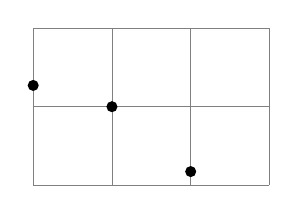
\begin{tikzpicture}
  \draw[help lines] (0,0) grid (3,2);
  \pgfpathcircle{\pgfpoint{1cm}{1cm}} {2pt}
  \pgfpathcircle{\pgfpoint{2cm}{5pt}} {2pt}
  \pgfpathcircle{\pgfpoint{0pt}{.5in}}{2pt}
  \pgfusepath{fill}
\end{tikzpicture}   
\end{codeexample}
\end{command}

\begin{command}{\pgfpointorigin}
  Yields the origin. Same as |\pgfpoint{0pt}{0pt}|.
\end{command}

\begin{command}{\pgfpointpolar\marg{degree}\marg{radius}}
  Yields a point location given in polar coordinates. You can specify
  the angle only in degrees, radians are not supported, currently.
\begin{codeexample}[]
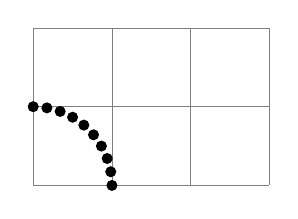
\begin{tikzpicture}
  \draw[help lines] (0,0) grid (3,2);

  \foreach \angle in {0,10,...,90}
    {\pgfpathcircle{\pgfpointpolar{\angle}{1cm}}{2pt}}
  \pgfusepath{fill}
\end{tikzpicture}   
\end{codeexample}
\end{command}



\subsection{Coordinates in the Xy- and Xyz-Coordinate Systems}

Coordinates can also be specified as multiples of an $x$-vector and a
$y$-vector. Normally, the $x$-vector points one centimeter in the
$x$-direction and the $y$-vector points one centimeter in the
$y$-direction, but using the commands |\pgfsetxvec| and
|\pgfsetyvec| they can be changed. Note that the $x$- and
$y$-vector do not necessarily point ``horizontally'' and
``vertically.''

It is also possible to specify a point as a multiple of three vectors,
the $x$-, $y$-, and $z$-vector. This is useful for creating simple
three dimensional graphics.

\begin{command}{\pgfpointxy\marg{$s_x$}\marg{$s_y$}}
  Yields a point that is situated at $s_x$ times the
  $x$-vector plus $s_y$ times the $y$-vector.
\begin{codeexample}[]
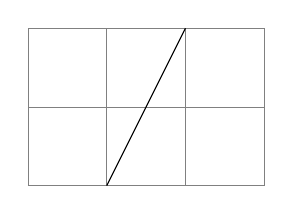
\begin{tikzpicture}
  \draw[help lines] (0,0) grid (3,2);
  \pgfpathmoveto{\pgfpointxy{1}{0}}
  \pgfpathlineto{\pgfpointxy{2}{2}}
  \pgfusepath{stroke}
\end{tikzpicture}   
\end{codeexample}
\end{command}

\begin{command}{\pgfpointxyz\marg{$s_x$}\marg{$s_y$}\marg{$s_z$}}
  Yields a point that is situated at $s_x$ times the
  $x$-vector plus $s_y$ times the $y$-vector plus  $s_z$ times the
  $z$-vector.
\begin{codeexample}[]
\begin{pgfpicture}
  \pgfsetarrowsend{to}
  
  \pgfpathmoveto{\pgfpointorigin}
  \pgfpathlineto{\pgfpointxyz{0}{0}{1}}
  \pgfusepath{stroke}
  \pgfpathmoveto{\pgfpointorigin}
  \pgfpathlineto{\pgfpointxyz{0}{1}{0}}
  \pgfusepath{stroke}
  \pgfpathmoveto{\pgfpointorigin}
  \pgfpathlineto{\pgfpointxyz{1}{0}{0}}
  \pgfusepath{stroke}
\end{pgfpicture}
\end{codeexample}
\end{command}


\begin{command}{\pgfsetxvec\marg{point}}
  Sets that current $x$-vector for usage in the $xyz$-coordinate
  system. 
  \example
\begin{codeexample}[]
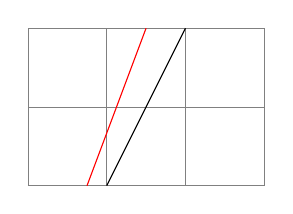
\begin{tikzpicture}
  \draw[help lines] (0,0) grid (3,2);
  
  \pgfpathmoveto{\pgfpointxy{1}{0}}
  \pgfpathlineto{\pgfpointxy{2}{2}}
  \pgfusepath{stroke}

  \color{red}
  \pgfsetxvec{\pgfpoint{0.75cm}{0cm}}
  \pgfpathmoveto{\pgfpointxy{1}{0}}
  \pgfpathlineto{\pgfpointxy{2}{2}}
  \pgfusepath{stroke}
\end{tikzpicture}   
\end{codeexample}
\end{command}

\begin{command}{\pgfsetyvec\marg{point}}
  Works like |\pgfsetyvec|.
\end{command}

\begin{command}{\pgfsetzvec\marg{point}}
  Works like |\pgfsetzvec|.
\end{command}




\subsection{Building Coordinates From Other Coordinates}

Many commands allow you to construct a coordinate in terms of other
coordinates.


\subsubsection{Basic Manipulations of Coordinates}

\begin{command}{\pgfpointadd\marg{$v_1$}\marg{$v_2$}}
  Returns the sum vector $\meta{$v_1$} + \meta{$v_2$}$.
\begin{codeexample}[]
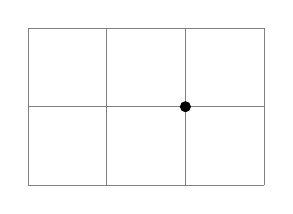
\begin{tikzpicture}
  \draw[help lines] (0,0) grid (3,2);
  \pgfpathcircle{\pgfpointadd{\pgfpoint{1cm}{0cm}}{\pgfpoint{1cm}{1cm}}}{2pt}
  \pgfusepath{fill} 
\end{tikzpicture}
\end{codeexample}
\end{command}

\begin{command}{\pgfpointscale\marg{factor}\marg{coordinate}}
  Returns the vector $\meta{factor}\meta{coordinate}$.
\begin{codeexample}[]
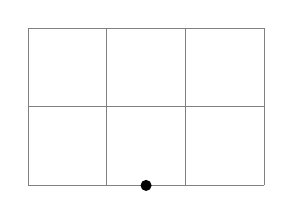
\begin{tikzpicture}
  \draw[help lines] (0,0) grid (3,2);
  \pgfpathcircle{\pgfpointscale{1.5}{\pgfpoint{1cm}{0cm}}}{2pt}
  \pgfusepath{fill} 
\end{tikzpicture}
\end{codeexample}
\end{command}

\begin{command}{\pgfpointdiff\marg{start}\marg{end}}
  Returns the difference vector $\meta{end} - \meta{start}$.
\begin{codeexample}[]
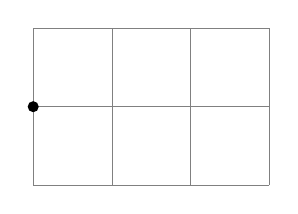
\begin{tikzpicture}
  \draw[help lines] (0,0) grid (3,2);
  \pgfpathcircle{\pgfpointdiff{\pgfpoint{1cm}{0cm}}{\pgfpoint{1cm}{1cm}}}{2pt}
  \pgfusepath{fill} 
\end{tikzpicture}
\end{codeexample}
\end{command}


\begin{command}{\pgfpointnormalised\marg{point}}
  This command returns a normalized version of \meta{point}, that is,
  a vector of length 1pt pointing in the direction of \meta{point}. If
  \meta{point} is the $0$-vector or extremely short, a vector of
  length 1pt pointing upwards is returned.

  This command is \emph{not} implemented by calculating the length of
  the vector, but rather by calculating the angle of the vector and
  then using (something equivalent to) the |\pgfpointpolar|
  command. This ensures that the point will really have length 1pt,
  but it is not guaranteed that the vector will \emph{precisely} point
  in the direction of \meta{point} due to the fact that the polar
  tables are accurate only up to one degree. Normally, this is not a
  problem.
\begin{codeexample}[]
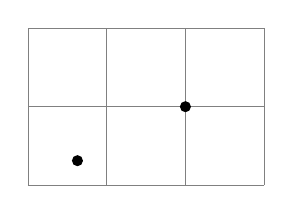
\begin{tikzpicture}
  \draw[help lines] (0,0) grid (3,2);
  \pgfpathcircle{\pgfpoint{2cm}{1cm}}{2pt}
  \pgfpathcircle{\pgfpointscale{20}
    {\pgfpointnormalised{\pgfpoint{2cm}{1cm}}}}{2pt}
  \pgfusepath{fill} 
\end{tikzpicture}
\end{codeexample}  
\end{command}


\subsubsection{Points Traveling along Lines and Curves}

\label{section-pointsattime}

The commands in this section allow you to specify points on a line or
a curve. Imaging a point ``traveling'' along a curve from some point
$p$ to another point $q$. At time $t=0$ the point is at $p$ and at
time $t=1$ it is at $q$ and at time, say, $t=1/2$ it is ``somewhere in
the middle.'' The exact location at time $t=1/2$ will not necessarily
be the ``halfway point,'' that is, the point whose distance on the
curve from $p$ and $q$ is equal. Rather, the exact location will
depend on the ``speed'' at which the point is traveling, which in
turn depends on the lengths of the support vectors in a complicated
manner. If you are interested in the details, please see a good book
on B�zier curves.



\begin{command}{\pgfpointlineattime\marg{time $t$}\marg{point $p$}\marg{point $q$}}
  Yields a point that is the $t$th fraction between $p$
  and~$q$, that is, $p + t(q-p)$. For $t=1/2$ this is the middle of
  $p$ and $q$.

\begin{codeexample}[]
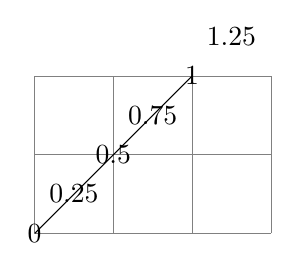
\begin{tikzpicture}
  \draw[help lines] (0,0) grid (3,2);
  \pgfpathmoveto{\pgfpointorigin}
  \pgfpathlineto{\pgfpoint{2cm}{2cm}}
  \pgfusepath{stroke}
  \foreach \t in {0,0.25,...,1.25}
    {\pgftext[at=
      \pgfpointlineattime{\t}{\pgfpointorigin}{\pgfpoint{2cm}{2cm}}]{\t}}
\end{tikzpicture}    
\end{codeexample}
\end{command}

\begin{command}{\pgfpointlineatdistance\marg{distance}\marg{start point}\marg{end point}}
  Yields a point that is located \meta{distance} many units removed
  from the start point in the direction of the end point. In other
  words, this is the point that results if we travel \meta{distance}
  steps from \meta{start point} towards \meta{end point}.
  \example
\begin{codeexample}[]
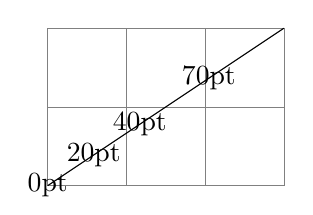
\begin{tikzpicture}
  \draw[help lines] (0,0) grid (3,2);
  \pgfpathmoveto{\pgfpointorigin}
  \pgfpathlineto{\pgfpoint{3cm}{2cm}}
  \pgfusepath{stroke}
  \foreach \d in {0pt,20pt,40pt,70pt}
    {\pgftext[at=
      \pgfpointlineatdistance{\d}{\pgfpointorigin}{\pgfpoint{3cm}{2cm}}]{\d}}
\end{tikzpicture}    
\end{codeexample}
\end{command}

\begin{command}{\pgfpointcurveattime\marg{time $t$}\marg{point
      $p$}\marg{point $s_1$}\marg{point $s_2$}\marg{point $q$}} 
  Yields a point that is on the B�zier curve from $p$ to $q$ with the
  support points $s_1$ and $s_2$. The time $t$ is used to determine
  the location, where $t=0$ yields $p$ and $t=1$ yields $q$.

\begin{codeexample}[]
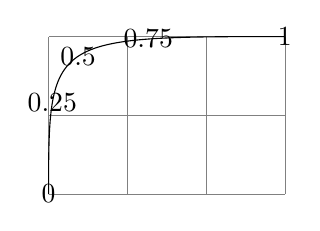
\begin{tikzpicture}
  \draw[help lines] (0,0) grid (3,2);
  \pgfpathmoveto{\pgfpointorigin}
  \pgfpathcurveto
    {\pgfpoint{0cm}{2cm}}{\pgfpoint{0cm}{2cm}}{\pgfpoint{3cm}{2cm}}
  \pgfusepath{stroke}
  \foreach \t in {0,0.25,0.5,0.75,1}
    {\pgftext[at=\pgfpointcurveattime{\t}{\pgfpointorigin}
                                         {\pgfpoint{0cm}{2cm}}
                                         {\pgfpoint{0cm}{2cm}}
                                         {\pgfpoint{3cm}{2cm}}]{\t}}
\end{tikzpicture}    
\end{codeexample}
\end{command}

\subsubsection{Points on Borders of Objects}

The following commands are useful for specifying a point that lies on
the border of special shapes. They are used, for example, by the shape
mechanism to determine border points of shapes.

\begin{command}{\pgfpointborderrectangle\marg{direction point}\marg{corner}}
  This command returns a point that lies on the intersection of a line
  starting at the origin and going towards the point \meta{direction
    point} and a rectangle whose center is in the origin and whose
  upper right corner is at \meta{corner}.

  The \meta{direction point} should have length ``about 1pt,'' but it
  will be normalized automatically. Nevertheless, the ``nearer'' the
  length is to 1pt, the less rounding errors.

\begin{codeexample}[]
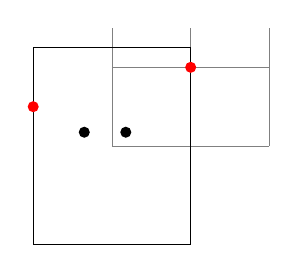
\begin{tikzpicture}
  \draw[help lines] (0,0) grid (2,1.5);
  \pgfpathrectanglecorners{\pgfpoint{-1cm}{-1.25cm}}{\pgfpoint{1cm}{1.25cm}}
  \pgfusepath{stroke}

  \pgfpathcircle{\pgfpoint{5pt}{5pt}}{2pt}
  \pgfpathcircle{\pgfpoint{-10pt}{5pt}}{2pt}
  \pgfusepath{fill}
  \color{red}
  \pgfpathcircle{\pgfpointborderrectangle
    {\pgfpoint{5pt}{5pt}}{\pgfpoint{1cm}{1.25cm}}}{2pt}
  \pgfpathcircle{\pgfpointborderrectangle
    {\pgfpoint{-10pt}{5pt}}{\pgfpoint{1cm}{1.25cm}}}{2pt}
  \pgfusepath{fill}
\end{tikzpicture}    
\end{codeexample}
\end{command}


\begin{command}{\pgfpointborderellipse\marg{direction point}\marg{corner}}
  This command works like the corresponding command for rectangles,
  only this time the \meta{corner} is the corner of the bounding
  rectangle of an ellipse.

\begin{codeexample}[]
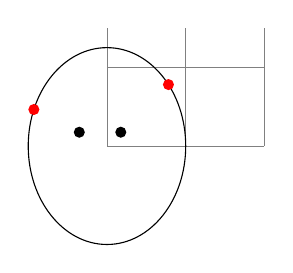
\begin{tikzpicture}
  \draw[help lines] (0,0) grid (2,1.5);
  \pgfpathellipse{\pgfpointorigin}{\pgfpoint{1cm}{0cm}}{\pgfpoint{0cm}{1.25cm}}
  \pgfusepath{stroke}

  \pgfpathcircle{\pgfpoint{5pt}{5pt}}{2pt}
  \pgfpathcircle{\pgfpoint{-10pt}{5pt}}{2pt}
  \pgfusepath{fill}
  \color{red}
  \pgfpathcircle{\pgfpointborderellipse
    {\pgfpoint{5pt}{5pt}}{\pgfpoint{1cm}{1.25cm}}}{2pt}
  \pgfpathcircle{\pgfpointborderellipse
    {\pgfpoint{-10pt}{5pt}}{\pgfpoint{1cm}{1.25cm}}}{2pt}
  \pgfusepath{fill}
\end{tikzpicture}    
\end{codeexample}
\end{command}


\subsubsection{Points on the Intersection of Lines}


\begin{command}{\pgfpointintersectionoflines\marg{$p$}\marg{$q$}\marg{$s$}\marg{$t$}}
  This command returns the intersection of a line going through $p$
  and $q$ and a line going through $s$ and $t$. If the lines do not
  intersection, an arithmetic overflow will occur.

\begin{codeexample}[]
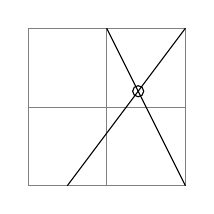
\begin{tikzpicture}
  \draw[help lines] (0,0) grid (2,2);
  \draw (.5,0) -- (2,2);
  \draw (1,2) -- (2,0);
  \pgfpathcircle{%
    \pgfpointintersectionoflines
      {\pgfpointxy{.5}{0}}{\pgfpointxy{2}{2}}
      {\pgfpointxy{1}{2}}{\pgfpointxy{2}{0}}}
    {2pt}
  \pgfusepath{stroke}
\end{tikzpicture}    
\end{codeexample}
\end{command}

\subsection{Extracting Coordinates}

There are two commands that can be used to ``extract'' the $x$- or
$y$-coordinate of a coordinate. 

\begin{command}{\pgfextractx\marg{dimension}\marg{point}}
  Sets the \TeX-\meta{dimension} to the $x$-coordinate of the point.

\begin{codeexample}[code only]
\newdimen\mydim
\pgfextractx{\mydim}{\pgfpoint{2cm}{4pt}}
%% \mydim is now 2cm
\end{codeexample}
\end{command}

\begin{command}{\pgfextracty\marg{dimension}\marg{point}}
  Like |\pgfextractx|, except for the $y$-coordinate.
\end{command}




\subsection{Internals of How Point Commands Work}

As a normal user of \pgfname\ you do not need to read this section. It
is relevant only if you need to understand how the point commands work
internally. 

When a command like |\pgfpoint{1cm}{2pt}| is called, all that happens
is that the two \TeX-dimension variables |\pgf@x| and |\pgf@y| are set
to |1cm| and |2pt|, respectively. A command like |\pgfpathmoveto| that
takes a coordinate as parameter will just execute this parameter and
then use the values of |\pgf@x| and |\pgf@y| as the coordinates to
which it will move the pen on the current path.

since commands like |\pgfpointnormalised| modify other variables
besides |\pgf@x| and |\pgf@y| during the computation of the final values of
|\pgf@x| and |\pgf@y|, it is a good idea to enclose a call of a
command like |\pgfpoint| in a \TeX-scope and then make the changes of
|\pgf@x| and |\pgf@y| global as in the following example:
\begin{codeexample}[code only]
...
{ % open scope
  \pgfpointnormalised{\pgfpoint{1cm}{1cm}}
  \global\pgf@x=\pgf@x % make the change of \pgf@x persist past the scope
  \global\pgf@y=\pgf@y % make the change of \pgf@y persist past the scope
}
% \pgf@x and \pgf@y are now set correctly, all other variables are
% unchanged 
\end{codeexample}

\makeatletter
Since this situation arises very often, the macro |\pgf@process| can
be used to perform the above code:
\begin{command}{\pgf@process\marg{code}}
  Executes the \meta{code} in a scope and then makes |\pgf@x| and
  |\pgf@y| global.
\end{command}

Note that this macro is used often internally. For this reason, it is
not a good idea to keep anything important in the variables |\pgf@x|
and |\pgf@y| since they will be overwritten and changed
frequently. Instead, intermediate values can ge stored in the
\TeX-dimensions |\pgf@xa|, |\pgf@xb|, |\pgf@xc| and their
|y|-counterparts |\pgf@ya|, |\pgf@yb|, |pgf@yc|. For example, here is
the code of the command |\pgfpointadd|:
\begin{codeexample}[code only]
\def\pgfpointadd#1#2{%
  \pgf@process{#1}%
  \pgf@xa=\pgf@x%
  \pgf@ya=\pgf@y%
  \pgf@process{#2}%
  \advance\pgf@x by\pgf@xa%
  \advance\pgf@y by\pgf@ya}
\end{codeexample}



%%% Local Variables: 
%%% mode: latex
%%% TeX-master: "pgfmanual"
%%% End: 
